\documentclass[11pt]{article}

\usepackage{fullpage}
\usepackage{amsmath}
\usepackage{graphicx}

\parindent 0pt
\parskip 7pt

\title{Text Classification: Report}
\author{David Storch (dstorch) \\ Matt Mahoney (mjmahone)}
\date{\today}

\begin{document}

\maketitle

\section{Feature distribution}

The average number of features for feature set 1 is 87.15 features per 
document. For feature set 2, there is an average of 47.95 features per 
document. In terms of distribution, feature set 1 is nicely distributed, 
with a large number of features appearing in only one document ($\sim$1400),
and fewer (by a logarithmic scale) features appearing in more documents.

For feature set 2, the distribution is fairly flat, with many features 
having appearing in 
between 800 and 5000 documents, but as there are
fewer features in feature set 2, it makes sense that the number of documents
with any specific frequency would be rather low.

\begin{center}
%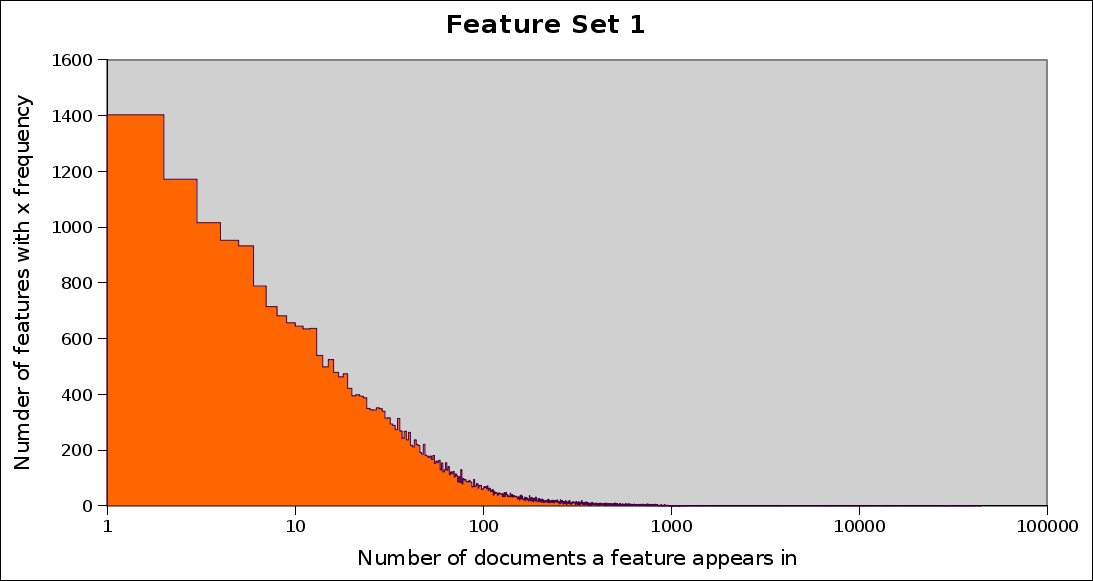
\includegraphics[bb=0 0 383 250]{../set1.png}
 % set1.png: 1093x581 pixel, 72dpi, 38.56x20.50 cm, bb=0 0 1093 581
\end{center}

\begin{center}
 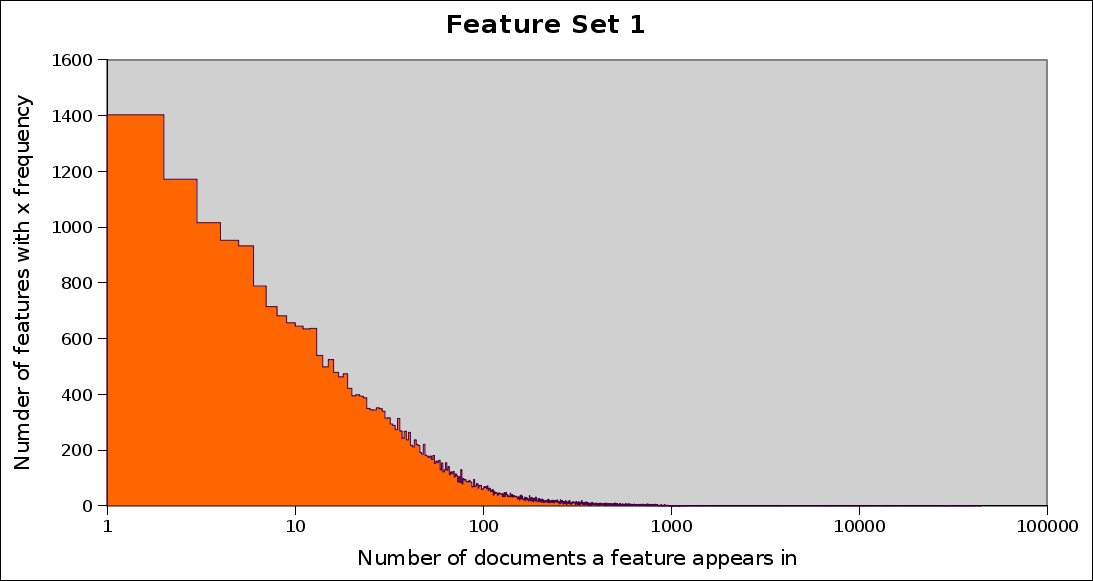
\includegraphics[width=15cm, height=9cm]{../set1.png}
 % set1.png: 1093x581 pixel, 72dpi, 38.56x20.50 cm, bb=0 0 1093 581
\end{center}

\begin{center}
 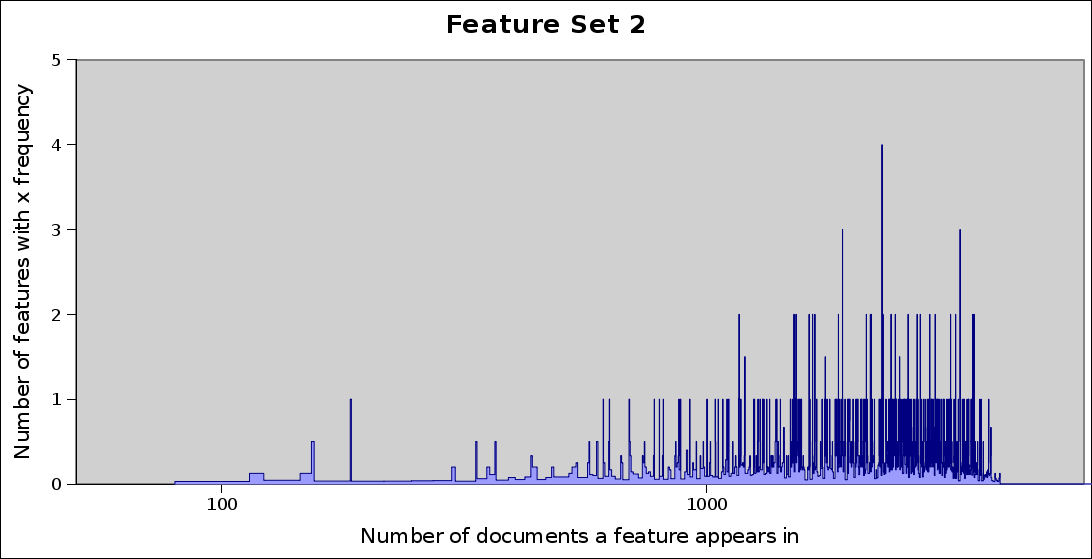
\includegraphics[width=15cm, height=9cm]{../set2.png}
 % set1.png: 1093x581 pixel, 72dpi, 38.56x20.50 cm, bb=0 0 1093 581
\end{center}

%\begin{center}
% 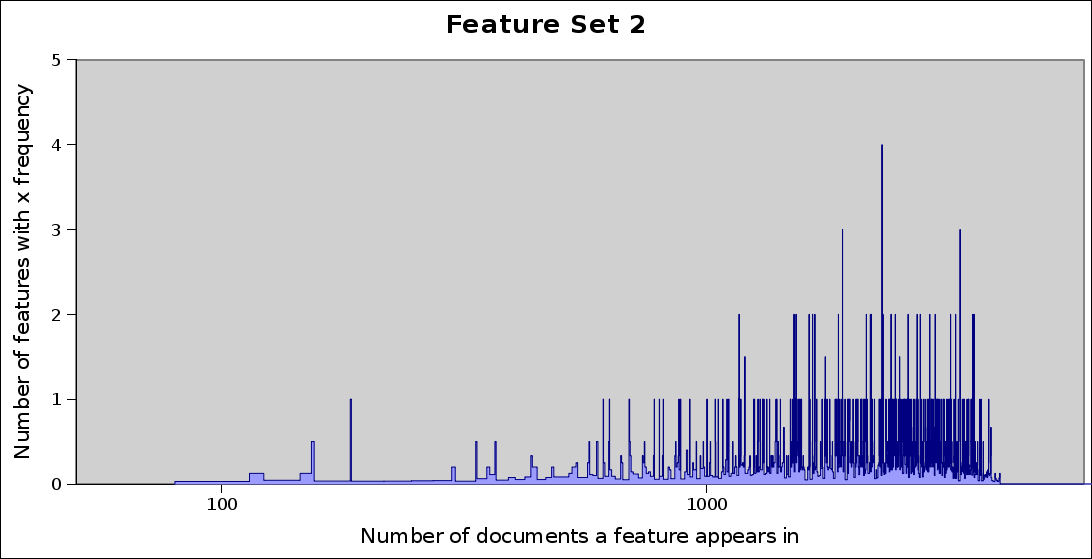
\includegraphics[bb=0 0 383 250]{../set2.png}
 % set2.png: 1092x559 pixel, 72dpi, 38.52x19.72 cm, bb=0 0 1092 559
%\end{center}


\section{Results from training set 1}

\centering
\begin{tabular}{r|c|c|c}
\textbf{Set to Classify} & \textbf{Feature Set} & \textbf{Multinomial Naive Bayes \%Error} &\textbf{Rocchio \%Error}\\
\hline
\texttt{training1.dat} & \texttt{features1.dat} & 14.37 & 72.10 \\
& \texttt{features2.dat} & 40.65 & 52.60 \\
\texttt{test.dat} & \texttt{features1.dat} & 39.57 & 74.56 \\
& \texttt{features2.dat} & 45.94 & 56.84 \\
\end{tabular}
\flushleft

\section{Explanation of results from \texttt{training1.dat}}

Since \texttt{training2.dat} has fewer features (but presumably more discriminating ones), we expect Rocchio
to perform better on this feature set---Rocchio depends on having distinct clusters of documents in the
high-dimensional vector space, and this is more likely to happen if the features are few but particular
to their class.

We expect Multinomial Naive Bayes to do better for \texttt{training1.dat} since it does not rely on
spatial clustering. For Bayes, having a larger number of (potentially less discriminating) features
helps to refine the Bayesian probability calculations. The data shows that MNB indeed has a slightly
reduced error rate for \texttt{training1.dat}.

\section{Results from training set 2}

\centering
\begin{tabular}{r|c|c|c}
\textbf{Set to Classify} & \textbf{Feature Set} & \textbf{Multinomial Naive Bayes \%Error} & \textbf{Rocchio \%Error} \\
\hline
\texttt{training2.dat} & \texttt{features1.dat} & 20.62 & 85.43 \\
& \texttt{features2.dat} & 75.93 & 71.93 \\
\texttt{test.dat} & \texttt{features1.dat} & 88.50 & 92.29\\
& \texttt{features2.dat} & 90.42 & 90.98 \\
\end{tabular}
\flushleft

\section{Explanation of results from \texttt{training2.dat}}

After inspecting some of the classifications in \texttt{training2.dat}, our subjective determinations of
the proper classification tends to differ from the provided classification. It is possible that the reduced
performance of both MNB and Rocchio is a result of bad training data. This is a particularly enticing conclusion because
the only difference between the numbers analyzed here and those from Questions 1 and 2 is the training set.

\section{Building a list of features}

Out motivation was the notion that discriminating features should appear frequently in one class compared to its appearances in
other classes. With this motivation in mind, our list of features was built by examining the documents in the union of
training set 1 and training set 2. We will denote this set of documents as $D$.
For each class $c$, we determined the total number of occurrences of each stemmed term $t \in D$.
Let this number of occurrences be denoted by freq$(c, t)$. We also found the total number of occurrences of each term $t$ in the entire
set $D$, which we will denote by tot$(t)$. Finally, for all term-class pairs $(t, c)$ we calculated the following ratio:

\centering
\begin{math}
R(t, c) = \dfrac{\text{freq}(t, c)}{\text{tot}(t)}
\end{math}
\flushleft

Our selection criterion was $R(t, c) \geq 0.3$ and $\text{tot}(t) \geq 10$---that is, the terms for which
at least 30\% of occurrences are in a single class and there are at least 10 occurrences in that class.
This produced a list of 1767 features.


\section{Results from \texttt{featuresADV.dat} and confusion matrix}

\centering
\begin{tabular}{r|c|c|c}
\textbf{Set to Classify} & \textbf{Feature Set} & \textbf{Multinomial Naive Bayes \%Error} & \textbf{Rocchio \%Error} \\
\hline
\texttt{training1.dat} & \texttt{featuresADV.dat} & 73.70 & 73.88 \\
\texttt{test.dat} & \texttt{featuresADV.dat} & 85.09 & 89.84 \\
\end{tabular}
\flushleft

The confusion matrix for Rocchio, run with training set \texttt{training1.dat} and
feature set \texttt{featuresADV.dat}, appears below. The rows give the expected
classification, and the column gives the classification assigned by Rocchio.
\footnote{The row and column heads are the class numbers, as defined in the
file \texttt{categories.dat}.}

\centering
\begin{tabular}{c|cccccccccccc|}
& \textbf{0} & \textbf{1}& \textbf{2} & \textbf{3} & \textbf{4} & \textbf{5} & \textbf{6} & \textbf{7}& \textbf{8} & \textbf{9} & \textbf{10} \\
\hline
\textbf{0} & 64& 5& 12& 5& 5& 13& 8& 3& 3& 8& 1 \\
\textbf{1}  & 42& 146& 70& 40& 26& 79& 74& 40& 46& 56& 13 \\
\textbf{2} & 9& 11& 89& 9& 7& 19& 10& 8& 9& 15& 6 \\
\textbf{3}  & 25& 27& 51& 96& 19& 63& 42& 31& 32& 32& 10 \\
\textbf{4}  & 37& 33& 74& 42& 90& 78& 48& 35& 47& 45& 10 \\
\textbf{5}  & 2& 6& 11& 4& 3& 66& 6& 9& 6& 4& 2 \\
\textbf{6}  & 16& 21& 30& 15& 7& 45& 117& 13& 10& 19& 11 \\
\textbf{7}  & 14& 7& 26& 14& 8& 28& 16& 83& 8& 13& 2 \\
\textbf{8}  & 23& 23& 44& 22& 13& 60& 32& 22& 119& 28& 5 \\
\textbf{9}  & 8& 5& 14& 4& 5& 19& 10& 6& 9& 83& 0 \\
\textbf{10}  & 63& 56& 117& 54& 41& 124& 83& 73& 55& 67& 70 \\
\end{tabular}
\flushleft

Similarly, the confusion matrix for Multinomial Naive Bayes is 

\centering
\begin{tabular}{c|cccccccccccc|}
& \textbf{0} & \textbf{1}& \textbf{2} & \textbf{3} & \textbf{4} & \textbf{5} & \textbf{6} & \textbf{7}& \textbf{8} & \textbf{9} & \textbf{10} \\
\hline
\textbf{0} & 32& 27& 4& 4& 16& 2& 2& 3& 13& 1& 25 \\
\textbf{1} & 13& 283& 12& 30& 62& 14& 9& 23& 63& 3& 137 \\
\textbf{2} & 9& 54& 37& 6& 19& 2& 1& 4& 20& 1& 40 \\
\textbf{3} & 17& 107& 4& 43& 64& 8& 7& 8& 54& 5& 121 \\
\textbf{4} & 16& 123& 15& 26& 159& 14& 9& 14& 62& 3& 101 \\
\textbf{5} & 3& 24& 0& 4& 12& 38& 5& 3& 7& 0& 24 \\
\textbf{6} & 9& 72& 6& 20& 46& 10& 24& 6& 50& 2& 65 \\
\textbf{7} & 9& 66& 2& 9& 25& 7& 5& 31& 28& 1& 41 \\
\textbf{8} & 13& 86& 8& 17& 56& 10& 4& 4& 105& 1& 100 \\
\textbf{9} & 5& 56& 3& 6& 18& 1& 3& 4& 23& 2& 46 \\
\textbf{10} & 22& 203& 24& 31& 94& 23& 16& 25& 86& 2& 298 \\
\end{tabular}
\flushleft

As evident from percent error statistics and our confusion matrices, using \texttt{featuresADV.dat} led to significantly
worse classification results compared to both Rocchio and Naive Bayes with \texttt{features1.dat} and
\texttt{features2.dat}\footnote{and using the same training set, \texttt{training1.dat}}. One probable cause is that \texttt{featuresADV.dat} is a
relatively small set ($\sim$1700 terms), and therefore some documents in the class might not contain many
of the features. Another possible cause is that the cutoff, $\text{tot}(t) \geq 10$, is too low. We are
allowing terms that might only appear 10 times in the class to be included. This means that, given the small
number of occurrences of the such terms, the $R(t, c) \geq 0.3$ lower bound might not be meaningful.


\end{document}
